% L12b student companion deck: why markets crash, on a Wolfram market with a rule switch.
%
% November 6, 2026: built from the rewritten lecture notebook, frame for frame. Notation
% follows the lecture: intention z_{j}(t) in {0,1,2} (Buy, Hold, Sell), neighbors \partial i,
% neighbor sum c_{i}(t) in {0,...,8}, table entries a_{c}, rule number, fraction f of
% switching traders, dealer net trade x_{t}, dealer shares Q_{t-1}, price P_{t}, depth h.
% No example parameters appear here (instructor rule, November 5, 2026).
\documentclass[aspectratio=169,11pt]{beamer}
\usepackage{vnslides}

\newcommand{\repo}{https://github.com/varnerlab/CHEME-5660-CourseRepository-Fall-2026/blob/main/lectures/week-12/L12b}

\title{\texorpdfstring{{\vnheavy L12b}}{L12b}: Why Do Markets Crash?}
\subtitle{CHEME 5660 Cornell University}
\author{Copyright Jeffrey Varner 2026. All Rights Reserved}

\begin{document}

\vntitlepage

\begin{frame}{Disclaimer and Risks}
  \vspace{0.6em}
  \textbf{\ink{Training only.}} This content is for training and informational
  purposes only. The teaching team does not make, give, or endorse any offer or
  solicitation to buy or sell securities or derivative products, or provide
  investment or trading advice or strategy.

  \vspace{1.1em}
  \textbf{\ink{Risk.}} Trading involves risk and is generally not recommended for
  those with limited resources, experience, or a low risk tolerance. Past
  performance does not guarantee future success.

  \vspace{1.1em}
  \textbf{\ink{Responsibility.}} You are responsible for your investment decisions
  based on your financial circumstances, objectives, risk tolerance, and
  liquidity needs.
\end{frame}

\begin{frame}{Objectives for Today}
  Today, we build a simple agent-based market and ask whether changing one entry
  of a trading rule can turn a calm market into a falling one.

  \vspace{0.5em}
  {\large\textbf{\ink{Today's concepts}}}
  \begin{itemize}\setlength{\itemsep}{0.4em}
    \item \hilite{Rules as policies}: a lookup table from what neighbors intend to
      what a trader intends next.
    \item \hilite{The dealer}: how net buying raises the price, net selling lowers
      it, and why a switched market needs a control.
    \item \hilite{Rule-switch simulation}: reading the selling fraction and the
      price, and what the comparison does not tell us about real crashes.
  \end{itemize}
\end{frame}

\begin{frame}{What You Need to Know}
  \vspace{0.3em}
  {\large\textbf{\ink{Core concepts}}}
  \begin{itemize}\setlength{\itemsep}{0.4em}
    \item A Wolfram rule maps the neighbor sum $c\in\{0,1,\dots,8\}$ to the
      trader's next intention. Rules 19280 and 19286 differ only at $c=1$: Buy
      versus Sell.
    \item The dealer sets the price from the net trade, so we compare every
      switched market with a control that shares its history.
    \item Giving the changed rule to a fraction $f$ of the traders can tip the
      market toward a Sell majority while the control does not. This is an
      analogy for crashes, not an explanation of them.
  \end{itemize}

  \vspace{0.5em}
  {\large\textbf{\ink{For understanding}} \dimmed{(you won't reproduce these)}}
  \begin{itemize}\setlength{\itemsep}{0.3em}
    \item The dealer's price update formula and the technical traders' band rule.
    \item The edge-trader conditions and the Q-learning notebook.
  \end{itemize}
\end{frame}

\begin{frame}{Lectures and Examples}
  \vspace{0.3em}
  {\normalsize\textbf{\ink{Lecture:}}\par\small
  \href{\repo/CHEME-5660-L12b-Lecture-WhyDoMarketsCrash-ABM-Fall-2026.ipynb}{\dimmed{CHEME-5660-L12b-Lecture-WhyDoMarketsCrash-ABM-Fall-2026.ipynb}}}

  \vspace{0.6em}
  {\normalsize\textbf{\ink{Example:}}\par\small
  \href{\repo/CHEME-5660-L12b-Example-Wolfram-RuleSwitch-Fall-2026.ipynb}{\dimmed{CHEME-5660-L12b-Example-Wolfram-RuleSwitch-Fall-2026.ipynb}}}

  \vspace{0.6em}
  Optional advanced notebooks are listed on the Optional Advanced Material frame.
\end{frame}

% ========== Why do markets crash?
\begin{frame}{Why Do Markets Crash?}
  A market crash is a sudden, significant decline in prices across a broad
  market. Three episodes show investor psychology swinging from euphoria to panic:
  \begin{center}
    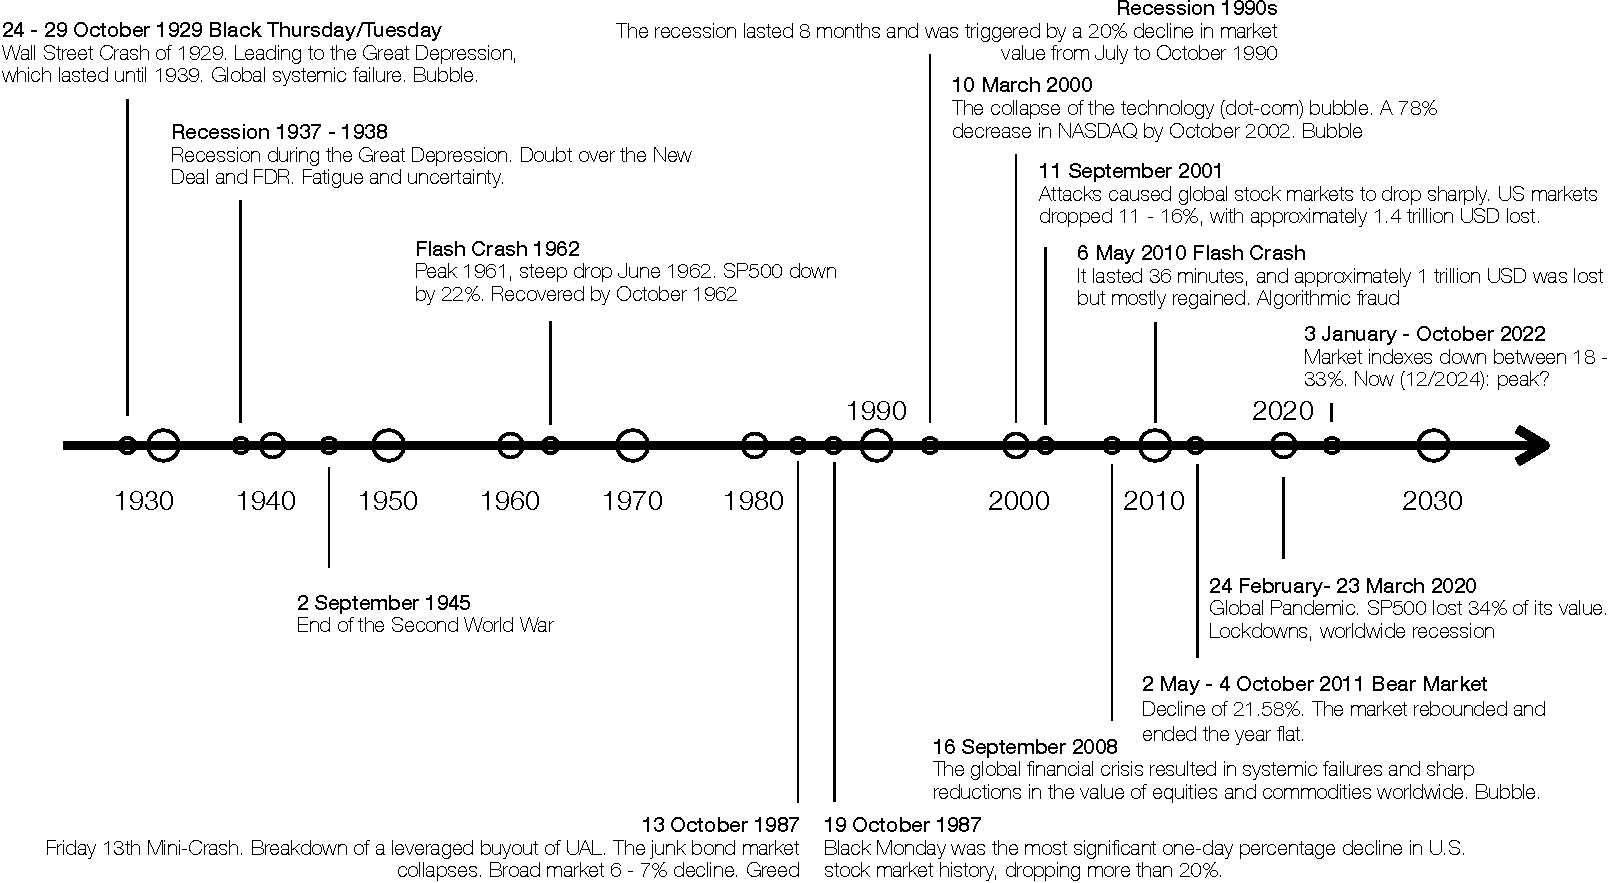
\includegraphics[width=\textwidth,height=0.62\textheight,keepaspectratio]{../figs/Fig-Crashes-Schematic-2024.pdf}
  \end{center}
\end{frame}

\begin{frame}{Three Landmark Episodes}
  Three episodes, each with a different trigger:
  \begin{itemize}\setlength{\itemsep}{0.5em}
    \item \hilite{1929 Wall Street Crash}: margin-fueled speculation met a sudden
      loss of confidence, and leveraged investors rushed to cover.
    \item \hilite{1987 Black Monday}: portfolio insurance and program trading
      amplified a slide, and a one-day 22.6\% Dow drop followed.
    \item \hilite{April 2025 tariff mini-crash}: tariff news and fast algorithmic
      selling hit sentiment first and fundamentals second.
  \end{itemize}
  \slidenote{Sources:}{\href{https://www.federalreservehistory.org/essays/stock-market-crash-of-1929}{\dimmed{Federal Reserve History}}; \href{https://fraser.stlouisfed.org/title/report-presidential-task-force-market-mechanisms-5732}{\dimmed{Brady Report}}; \href{https://ustr.gov/about-us/policy-offices/press-office/press-releases/2025/april}{\dimmed{USTR}}}
\end{frame}

\begin{frame}{Agent-Based Modeling of Market Crashes}
  Markets are man-made systems, and they can fail. An \hilite{agent-based model}
  simulates traders as autonomous agents with their own rules, and the price
  emerges from their actions:
  \begin{itemize}\setlength{\itemsep}{0.5em}
    \item \hilite{Iori (2002)}: interacting traders who imitate each other
      produce large fluctuations and volatility clustering.
    \item \hilite{Lux--Marchesi (1999)}: agents switch between fundamentalist and
      chartist strategies, producing bubbles and crashes.
  \end{itemize}
  Today, traders sit on a grid and act on what their neighbors intend to do.
  \slidenote{Sources:}{\href{https://arxiv.org/abs/adap-org/9905005}{\dimmed{Iori}}; \href{https://doi.org/10.1038/17290}{\dimmed{Lux and Marchesi, Nature 397}}}
\end{frame}

% ========== Agents as Policies
\begin{frame}{Agents as Policies}
  A \hilite{policy} is a table that gives, for each possible state of an agent's
  surroundings, the action the agent takes. In our market:
  \begin{itemize}\setlength{\itemsep}{0.5em}
    \item \hilite{State}: a number summarizing what a trader's four neighbors intend.
    \item \hilite{Action}: the trader's own next intention, Buy, Hold, or Sell.
    \item \hilite{Source of the table}: Q-learning could learn it from experience.
      Our traders are handed their tables, and we change one entry.
  \end{itemize}
\end{frame}

% ========== Wolfram Markets
\begin{frame}{Wolfram Markets}
  Traders sit on the cells of a square grid, and simple local rules produce
  market-level behavior, as in Wolfram's cellular automata:
  \begin{itemize}\setlength{\itemsep}{0.5em}
    \item \hilite{Intention}: Buy, Hold, or Sell, coded $0$, $1$, $2$. We write
      $z_{j}(t)\in\{0,1,2\}$ for the intention of trader $j$ at step $t$.
    \item \hilite{Neighbors}: an interior trader has four, above, below, left,
      and right, and updates its intention from theirs.
  \end{itemize}
  This is a three-color two-dimensional cellular automaton.
  \slidenote{Source:}{\href{https://github.com/varnerlab/Wolfram-markets-abm-paper}{\dimmed{our paper on rule switches in Wolfram markets}}; Wolfram, \emph{A New Kind of Science} (2002), Chapter 3}
\end{frame}

\begin{frame}{The Neighbor Sum}
  Let $\partial i$ denote the four neighbors of trader $i$. The trader looks only
  at the \hilite{neighbor sum} $c_{i}(t)$, not at its own current intention:
  \begin{equation*}
    \underbrace{c_{i}(t)}_{\text{neighbor sum}} = \sum_{j\in\partial i}z_{j}(t)\in\{0,1,\dots,8\}
  \end{equation*}
  The policy is a table with one action $a_{c}\in\{0,1,2\}$ for each of the nine
  sums $c=0,1,\dots,8$: the intention the trader adopts next when its neighbor
  sum is $c$.
\end{frame}

\begin{frame}{Rule Numbers}
  There are $3^{9}=19{,}683$ such tables. We identify each by its \hilite{rule
  number}, the table written in base 3, with digits from $a_{8}$ on the left to
  $a_{0}$ on the right:
  \begin{equation*}
    \underbrace{\sum_{c=0}^{8}a_{c}\,3^{c}}_{\text{rule number}}
  \end{equation*}
  We use Rule 19280, $(222110002)_{3}$, as the baseline.
\end{frame}

\begin{frame}{Edge Traders and One Simulation Step}
  Some edge traders are \hilite{technical traders}: they Buy when the dealer's
  price falls below a band around its recent average, Sell above it, and Hold
  otherwise. The others stay in Hold. Each step runs in this order:
  \begin{enumerate}\setlength{\itemsep}{0.35em}
    \item \hilite{Rule changes and orders}: apply any scheduled rule change; traders
      order from their intentions.
    \item \hilite{Clearing}: the dealer matches orders and updates the price.
    \item \hilite{Technical traders}: update their bands and intentions.
    \item \hilite{Interior traders}: all update together from the previous
      intentions of their neighbors.
  \end{enumerate}
\end{frame}

% ========== The Rule Switch
\begin{frame}{The Rule Switch}
  Rule 19286, $(222110022)_{3}$, differs from the baseline in one entry. Three
  neighbors intend Buy and one Hold, so $c=1$: Rule 19280 buys, and Rule 19286 sells:
  \begin{center}
    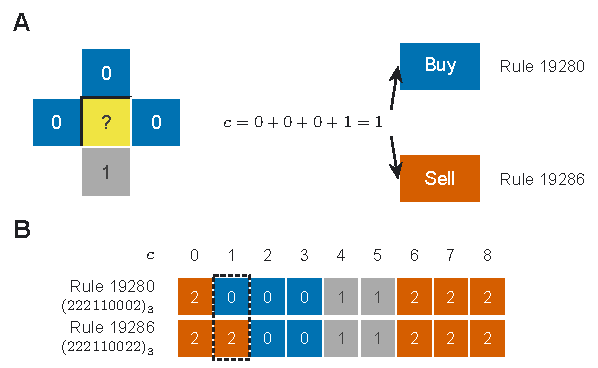
\includegraphics[width=\textwidth,height=0.62\textheight,keepaspectratio]{../figs/Fig-L12b-RuleSwitch.pdf}
  \end{center}
\end{frame}

\begin{frame}{The Rule-Switch Experiment}
  We use the one-entry difference as a model of a change in psychology. The
  experiment has three parts:
  \begin{itemize}\setlength{\itemsep}{0.5em}
    \item \hilite{Shared history}: all interior traders follow Rule 19280. At the
      switch step, a fraction $f$ of them, chosen in advance, receive Rule 19286
      and keep their intentions, cash, and shares.
    \item \hilite{Control}: a second market with the same history never switches,
      so differences after the switch come from the rule change.
    \item \hilite{Edge traders}: in the active condition they react to the price;
      in the held condition they stay in Hold.
  \end{itemize}
\end{frame}

\begin{frame}{Example: Rule Switch}
  \vspace{0.3em}
  {\normalsize\textbf{\ink{Example:}}\par\small
  \href{\repo/CHEME-5660-L12b-Example-Wolfram-RuleSwitch-Fall-2026.ipynb}{\dimmed{CHEME-5660-L12b-Example-Wolfram-RuleSwitch-Fall-2026.ipynb}}}

  \vspace{0.8em}
  In this example, we plot the fraction of traders who intend to sell and the
  dealer's price for a switched market beside its control.

  \vspace{0.8em}
  The example uses the dealer's price throughout, so next we look at how the
  dealer sets it.
\end{frame}

% ========== Prices and the Dealer
\begin{frame}{Prices and the Dealer}
  The dealer holds cash and shares and takes the other side of trades the traders
  do not match. At step $t$, $x_{t}$ is the net number of shares the dealer sells
  to traders (positive for net buyers), $Q_{t-1}$ the dealer's shares before the
  trade, and $P_{t-1}$ the price before it. The price after the trade is:
  \begin{equation*}
    P_{t} = P_{t-1}\Bigl(\underbrace{\frac{Q_{t-1}}{Q_{t-1}-x_{t}}}_{\substack{\text{shares before}\\\text{over shares after}}}\Bigr)^{2}
  \end{equation*}
  Net buyers, $x_{t}>0$: the ratio exceeds one and the price rises. Net sellers,
  $x_{t}<0$: the ratio is below one and the price falls.
\end{frame}

\begin{frame}{Dealer Depth and Public Intentions}
  \vspace{0.3em}
  \begin{itemize}\setlength{\itemsep}{0.5em}
    \item \hilite{Depth}: the dealer's depth $h$ is its initial shares per trader.
      A deeper dealer holds more shares $Q_{t-1}$, so a net order moves
      the price less.
    \item \hilite{Public intentions}: neighbors read an intention without
      checking holdings, so it can spread even when its sender cannot trade.
    \item \hilite{Control}: a shallow dealer can crash the price with no switch at
      all, so we read a switched price beside its control's.
  \end{itemize}
  \slidenote{Details:}{the full clearing rule is in the example's code and in the paper}
\end{frame}

% ========== Back to Real Crashes
\begin{frame}{Back to Real Crashes}
  Our market is a toy, and we do not claim it explains any real crash. The rule
  switch is a loose analogy:
  \begin{itemize}\setlength{\itemsep}{0.5em}
    \item \hilite{1929}: buying neighborhoods ($c=1,2,3$) sustain themselves; the
      switched entry sells when one neighbor holds back, confidence turning.
    \item \hilite{1987}: portfolio insurance told some investors to sell; here a
      fraction $f$ of traders receive a different entry.
    \item \hilite{April 2025}: news changed how traders read each other, so the
      same neighborhood leads to a different action.
  \end{itemize}
\end{frame}

% ========== Optional advanced material
\begin{frame}{Optional Advanced Material}
  \vspace{0.4em}
  {\normalsize\textbf{\ink{Q-learning:}} \dimmed{advanced/qlearning/}\par
  \href{\repo/advanced/qlearning/CHEME-5660-L12b-Advanced-QLearning-Fall-2026.ipynb}{\dimmed{CHEME-5660-L12b-Advanced-QLearning-Fall-2026.ipynb}}}

  \vspace{0.6em}
  How could a trader learn a policy table from experience instead of being handed
  one? We write the Q-learning update, lay out the algorithm, and describe when
  it converges to the best policy. Not a prerequisite for L13a.
\end{frame}

\begin{frame}{Summary}
  \vspace{0.3em}
  We built a simple agent-based market and used it to ask how a small change in
  trader behavior can tip a market toward selling.

  \vspace{0.4em}
  {\large\textbf{\ink{Key takeaways}}}
  \begin{itemize}\setlength{\itemsep}{0.4em}
    \item \hilite{Rules as policies}: a rule is a lookup table, and one entry can
      change.
    \item \hilite{Dealer and control}: net trades set the price, and a control
      isolates the switch.
    \item \hilite{Tipping, by analogy}: a switch for some traders can tip the
      market toward selling, but a simulation does not establish real causes.
  \end{itemize}
  \vspace{0.3em}
  Agent-based models ask how individual rules add up to market behavior.
\end{frame}

\end{document}
